\section{Schedules and the law}\label{to:sec:law}\label{sec:law}

Unless a result states an exception, the contract of Section~\ref{sec:contract} applies; Table~\ref{to:tab:contract} below collects it.

\begin{definition}[Schedule]\label{to:def:schedule}
A schedule $S$ is a finite, ordered list of arrival and release events. A visit $v$ brings a carrier $P_v$ with Hamiltonian $H_v$ into the device at its arrival and returns the same carrier, with the same Hamiltonian, at its release. Visits of the same carrier cannot overlap; visits of different carriers may overlap, and releases may come in any order. The device can act on a carrier only during its visit. A later loan of a carrier that the observer owns is a new visit, and its state may be correlated with everything the observer holds. The observer supplies the carriers and may choose them adaptively, using only outputs already released, its own memory and its quantum references; every receipt or message the observer sees is written on a carrier the observer has supplied, and its delivery is that carrier's release.
\end{definition}

Batch operation is the schedule in which every input arrives before any output is released; real time is the schedule in which input $t+1$ arrives only after output $t$ has left; a process with memory interleaves the two.

\begin{definition}[The schedule functional]\label{to:def:functional}
A \emph{private extension} of a target strategy $T$ on $S$ consists of an initial device state $\tau$, an inert purification $F$ of it that is never acted on, and unitaries on the device and the carriers present, following $S$, whose marginal strategy is within $\varepsilon$ of $T$ in the strategy distance, the largest trace distance over adaptive testers. These unitaries need not conserve energy; the extension is a mathematical object. For a purified tester $t$, an observer allowed by the schedule that keeps its initial purifying systems and everything it discards coherently, let $Z$ be everything it owns at the end, including these systems, its references and every released carrier, with no duplicate copy of a carrier loaned again; the tester starts independent of the device and of $F$. Let $E_t=\sum_v[\Tr H_v\rho_{v,\mathrm{release}}-\Tr H_v\rho_{v,\mathrm{arrival}}]$ be the energy handed over. Set
\[
k_{S,\varepsilon}(T)=\inf_{\text{private extensions}}\ \sup_{\text{purified }t}\Bigl[\tfrac{\ln2}\beta S(Z|F)_t+E_t\Bigr],
\]
and let $K_\beta^S(T)=\beta\,\bar k^S(T)/\ln2$, where $\bar k^S(T)=\inf_{\varepsilon_n\to0}\limsup_n k_{S_n,\varepsilon_n}(T_n)/n$ is the regularized rate along the block schedules $S_n$. As a check of the normalization, resetting a maximally mixed bit with zero Hamiltonian gives $k=\kB T\ln2$.
\end{definition}

Because the tester is purified and starts independent of the device, the final state of $F$, the device and $Z$ is pure, so $S(Z|F)=S(\omega)-S(\tau)$, with $\omega$ the device's final state, is the entropy the extension adds to its own record: the device cannot read $F$, and the same tester supplies both the entropy and the energy term. The purification is needed. For the identity channel on a qubit with zero Hamiltonian, run by a device that does nothing, a tester that feeds $I/2$ and keeps no purifier would be charged $S(Z|F)=1$ although the device adds no entropy; with the purifier in $Z$, $S(Z|F)=0$.

\begin{table}[tbp]
\centering
\small
\begin{tabular}{@{}>{\raggedright\arraybackslash}p{2.6cm}>{\raggedright\arraybackslash}p{12.2cm}@{}}
\toprule
Part of the contract & What it requires\\
\midrule
Target & A finite strategy on a specified schedule, such as a channel, a process or a delayed release, required of every observer, including inputs entangled with references the observer keeps.\\
Access & Inputs arrive and outputs are released as the schedule says; the observer chooses later inputs using released outputs, its memory and its references.\\
Ports & Each visit returns the same carrier with the Hamiltonian it arrived with. New or retired carriers need an inventory term, and changed Hamiltonians need a physical switch (Section~\ref{to:sec:law}).\\
Free dynamics & Unitaries that conserve the energy of the systems they act on, and Gibbs reservoirs at one temperature, declared in advance.\\
Controller & Returns approximately: its joint state with everything else ends close to its initial state tensored with the rest, and its actual mean energy and entropy each change by $o(n)$. Its startup capital is declared and may grow with $n$; it is not part of the rate.\\
Battery & Mechanical, with entropy change $o(n)$. Deterministic work: it starts in an energy eigenstate and ends in a fixed level with probability tending to one, with mean absolute deviation $o(n)$.\\
Limit & The error over the whole block of $n$ uses tends to zero, and the rate is per use as $n\to\infty$. Devices may have any size and running time, and the constructions are built for a number $n$ of uses known in advance. A rate of zero does not mean that a finite device runs at zero cost.\\
\bottomrule
\end{tabular}
\caption{The operational contract of Theorem~\ref{to:thm:law}. Appendix~\ref{to:app:schedules} states it in full.}\label{to:tab:contract}
\end{table}

\begin{table}[tbp]
\centering
\small
\begin{tabular}{@{}>{\raggedright\arraybackslash}p{4.6cm}>{\raggedright\arraybackslash}p{10.2cm}@{}}
\toprule
Results & What changes\\
\midrule
Real-time channel laws (Theorems~\ref{thm:main-realtime} and~\ref{thm:main-dichotomy}, Appendix~\ref{app:channels}) & Deterministic work allows a signed mean deviation of the battery from its final level, a weaker requirement than the absolute deviation; the lower bounds hold under either, and the constructions are claimed only under the signed one.\\
Strong converse of Theorem~\ref{thm:main-realtime} & The controller starts in its Gibbs state; a controller with a broad energy bank can break the converse (Remark~\ref{sw:rem:thermal-controller}).\\
Clock size (Theorem~\ref{thm:main-heisenberg}(b), Propositions~\ref{kt:prop:broadclock} and~\ref{kt:prop:clocksize}) & Hold at any work. The battery starts in a state that commutes with its Hamiltonian, and the vanishing-error bounds also ask the controller to return independently of everything else, within $\eta_n$, uniformly over inputs.\\
Fiber law (Theorem~\ref{thm:classes}) & Zero Hamiltonians, and a promise on the admissible inputs that is part of the task.\\
Two-qubit certificate (Proposition~\ref{to:prop:certificate}) & One episode, with finite budgets $P$ for the controller and the battery in place of the $o(n)$ terms.\\
Lent arm of Section~\ref{sec:protocol} & The observer returns the loan unmodified, jointly with the rest.\\
Comparisons of Section~\ref{to:sec:beyond} & Their own free operations, currencies and output inventory.\\
Exact return and zero error (rows of Table~\ref{to:tab:corollaries}) & Outside the contract; listed for comparison.\\
\bottomrule
\end{tabular}
\caption{Where a result departs from the default contract of Section~\ref{sec:contract} and Table~\ref{to:tab:contract}.}\label{tab:exceptions}
\end{table}

\FloatBarrier
\begin{theorem}[Work law for schedules]\label{to:thm:law}
Fix a temperature $0<T<\infty$, and let $S_n$ be the schedule of a block of $n$ uses, with the order of events across uses specified, in which each visit returns the same carrier with an unchanged Hamiltonian. The optimal rate of deterministic work for a device that returns its controller approximately is
\[
W^S=\frac{\ln2}{\beta}\,K_\beta^S.
\]
The lower bound holds for every implementation; the rate is attained using the finite-source and phase modules of Appendix~\ref{app:module}. Appendix~\ref{to:app:schedules} states the full contract, including the battery's absolute energy deviation. Resources that start correlated with the controller and must be returned in a prescribed joint state are not covered.
\end{theorem}


\subsection{The lower bound in one page}\label{sec:lowerbound}

The lower bound of Theorem~\ref{to:thm:law} is an accounting identity, and it is short enough to give here in full. The identity is a multipartite form of the finite-reservoir entropy-production identity of Esposito, Lindenberg and Van den Broeck and of Reeb and Wolf~\cite{EspositoLindenbergVandenBroeck10,ReebWolf14}; the step specific to the law is the identification $A=S(Z|F)$ below, against every observer. Entropies in this subsection are in nats.

\begin{lemma}[Whole-block identity]\label{lem:identity}
Let the device $D=CWR$ start in $\alpha_C\otimes|w\rangle\langle w|\otimes\gamma_R$, with $\gamma_R$ the Gibbs state of $R$ at inverse temperature $0<\beta<\infty$, independent of the observer, and run any sequence of energy-conserving unitaries on itself and the carriers present, following the schedule. For every purified observer, let $A=S(D_f)-S(D_i)$ be the entropy gained by the device, $E_t=\sum_v[\Tr H_v\rho_{v,\mathrm{release}}-\Tr H_v\rho_{v,\mathrm{arrival}}]$ the energy handed over on the carriers, and $I(C{:}W{:}R)_f=S(C_f)+S(W_f)+S(R_f)-S(D_f)$ the final total correlation among the device's parts. Then
\begin{equation}\label{eq:identity}
-\Delta E_W-\Delta E_C+\frac{\Delta S_C+S(W_f)}{\beta}
=E_t+\frac{A+D(\rho_{R_f}\|\gamma_R)+I(C{:}W{:}R)_f}{\beta}.
\end{equation}
\end{lemma}
\begin{proof}
Three identities and one conservation law. First, since the initial state is a product with a pure battery, $S(D_i)=S(C_i)+S(R_i)$, so
\[
A=\Delta S_C+S(W_f)+\Delta S_R-I(C{:}W{:}R)_f .
\]
Second, with $\gamma_R=e^{-\beta H_R}/Z_R$ and $\ln Z_R=S(\gamma_R)-\beta\Tr H_R\gamma_R$,
\[
D(\rho_{R_f}\|\gamma_R)=-S(R_f)+\beta\Tr H_R\rho_{R_f}+\ln Z_R
\quad\Longrightarrow\quad
\Delta S_R=\beta\,\Delta E_R-D(\rho_{R_f}\|\gamma_R).
\]
Third, every gate conserves the energy of the systems it acts on, so over the whole block
\[
\Delta E_C+\Delta E_W+\Delta E_R+E_t=0 .
\]
Substituting the second identity into the first, solving for $\Delta E_R$, and inserting it into the conservation law gives~\eqref{eq:identity}.
\end{proof}

Every term on the right of~\eqref{eq:identity} except $E_t$ and $A$ is nonnegative: relative entropy and total correlation are. The left side is the free energy drawn from the battery and the controller. Under the return rule of Section~\ref{sec:contract}, $|\Delta E_C|$, $|\Delta S_C|$ and $S(W_f)$ are $o(n)$, and the battery's nominal debit differs from $-\Delta E_W$ by its mean absolute deviation, also $o(n)$. So
\begin{equation}\label{eq:lower}
\text{nominal work}\ \ge\ E_t+\frac{A}{\beta}-o(n)
\end{equation}
for every observer. It remains to identify $A$ with the schedule functional. Purify the device's initial state by an inert register $F$, which no gate touches, and purify the observer. At the end of the block the global state of $F$, the device and the observer's systems $Z$ is pure, so $S(D_f)=S(ZF)$ and $S(D_i)=S(F)$, whence $A=S(Z|F)$. The actual device, with energy conservation forgotten, is a legal private extension of the target at the device's error, so $\sup_t[S(Z|F)_t/\beta+E_t]\ge k_{S,\varepsilon}$ and~\eqref{eq:lower} becomes nominal work $\ge k_{S,\varepsilon}(T)-o(n)$. Regularizing along the block schedules gives $W^S\ge(\ln2/\beta)K_\beta^S$. The argument uses neither time covariance nor exact return, and it needs no continuity estimate in the norm of any Hamiltonian; Appendix~\ref{to:app:schedules} states it with explicit budgets.

The identity also explains the figure of merit. The device cannot read $F$, so $S(Z|F)$ is exactly the entropy the implementation adds to its own record, and the same observer supplies both the entropy and the energy term. Nothing about speed enters: the identity holds for any number of gates and any running time.

\subsection{The upper bound in outline}\label{sec:upperbound}

For a near-optimal private extension, the construction records the observer's strategy from the arriving carriers on a rare branch of small probability; the gap between the worst observer and the actual one then becomes the expectation of one fixed positive operator on the device's records, and that gap is paid as heat by rare excitations of high-gap thermal qubits, so that every observer is charged the same work. Each release removes from the device's reach whatever its record shares with the released carrier, which is why the record is kept coherently and never measured.

Windows that collect a bundle of carriers and release it without feedback reduce exactly to the interleaved processes of Appendix~\ref{app:module}. General schedules, with overlapping visits, out-of-order releases and correlated re-entry, need the record to be kept on the actual carriers; the positive operator is obtained by duality on the cone of testers and acts, just before the last release, only on records the device still holds (Appendix~\ref{to:app:schedules}). The construction neither identifies the observer by tomography nor measures the ordinary history, and it never touches a released carrier. The proof of attainability uses its parts in this order (Figure~\ref{to:fig:ledger}): a private extension; the coherent recorder and the dual on the tester cone; the positive heat correction; the finite-source cache, which forms the required initial state from Gibbs supplies; the energy-conserving lift of the whole history; and separate refunds of the controller's actual energy and entropy, with the battery's entropy and absolute deviation kept sublinear (Appendix~\ref{app:module}).

\begin{figure}[t]
\centering
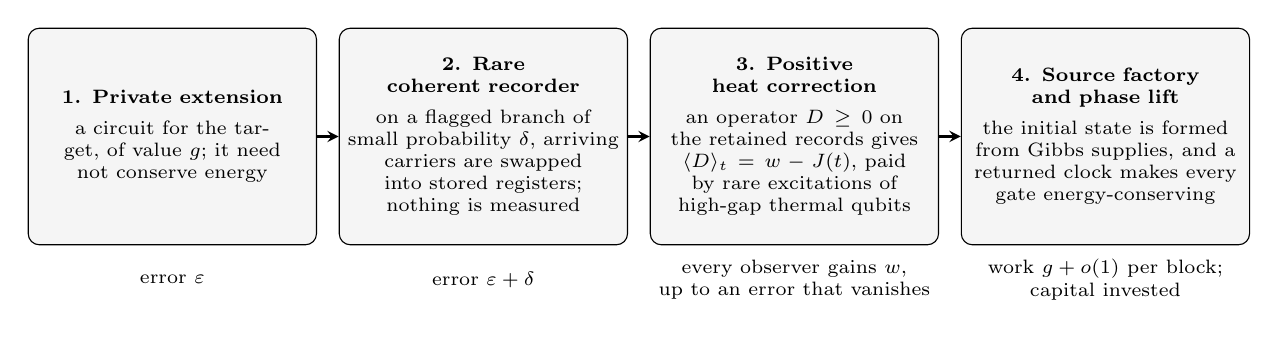
\begin{tikzpicture}[>=stealth, font=\scriptsize, stage/.style={draw, rounded corners, fill=gray!8, text width=3.45cm, align=center, minimum height=2.75cm, inner sep=3pt, anchor=north}]
  \node[stage] (s1) at (0,0) {\textbf{1. Private extension}\\[3pt] a circuit for the target, of value $g$; it need not conserve energy};
  \node[stage] (s2) at (3.95,0) {\textbf{2. Rare}\\\textbf{coherent recorder}\\[3pt] on a flagged branch of small probability $\delta$, arriving carriers are swapped into stored registers; nothing is measured};
  \node[stage] (s3) at (7.9,0) {\textbf{3. Positive heat correction}\\[3pt] an operator $D\ge0$ on the retained records gives $\langle D\rangle_t=w-J(t)$, paid by rare excitations of high-gap thermal qubits};
  \node[stage] (s4) at (11.85,0) {\textbf{4. Source factory and phase lift}\\[3pt] the initial state is formed from Gibbs supplies, and a returned clock makes every gate energy-conserving};
  \draw[->, thick] (s1) -- (s2); \draw[->, thick] (s2) -- (s3); \draw[->, thick] (s3) -- (s4);
  \node[align=center] at (0,-3.2) {error $\varepsilon$};
  \node[align=center] at (3.95,-3.2) {error $\varepsilon+\delta$};
  \node[align=center] at (7.9,-3.2) {every observer gains $w$,\\up to an error that vanishes};
  \node[align=center] at (11.85,-3.2) {work $g+o(1)$ per block;\\capital invested};
\end{tikzpicture}
\caption{The construction behind the upper bound of Theorem~\ref{to:thm:law}, read as a ledger (Appendix~\ref{to:app:schedules}). The record in stage~2 is coherent: no history is measured or postselected, and the rare branch adds only a small error. Stage~3 makes the unused part of the worst-case budget, $w-J(t)$ for the observer $t$, a positive effect on systems the device still holds, so every observer is charged the same work. Stage~4 is the finite-source and phase module of Appendix~\ref{app:module}; its capital can be enormous, but it is invested, not consumed, and comes back with the controller.}
\label{to:fig:ledger}
\end{figure}

Two remarks fix the scope for schedules that change their carriers.

\paragraph{New and retired carriers.} A schedule that delivers new output carriers, or retires inputs, needs the inventory term $(\sum_{\mathrm{new}}\ln Z_O-\sum_{\mathrm{retired}}\ln Z_I)/\beta$ in the functional; without it even the preparation of a thermal state is mispriced. The lower bound with this term holds for every schedule, since the accounting identity changes the stock's partition function by exactly this amount. In batch, for a time-covariant channel $\Phi_{A\to B}$, the corrected formula is a theorem: the capacity theorem~\cite[Thm.~7.1]{FBB21}, applied to the time-covariant channel $X_{AB}\mapsto\gamma_A\otimes\Phi(\Tr_BX_{AB})$ on the fixed composite system $AB$ with Hamiltonian $H_A+H_B$, attains it, because the capacity of that channel is $\sup_\sigma[D(\Phi(\sigma)\|\gamma_B)-D(\sigma\|\gamma_A)]$. Faist, Berta and Brand\~ao define the capacity of a channel between different systems with the unnormalized operators $e^{-\beta H}$~\cite[Eq.~(4.2)]{FBB21}, which gives this expression plus $\ln(Z_A/Z_B)$; the two differ only in how the partition functions of created and discarded systems are booked, which our contract charges through the inventory term. For general schedules with new or retired carriers, a matching construction depends on a source-formation step that we do not prove here.

\paragraph{Changing Hamiltonians.} Changes of Hamiltonian are not free relabellings: after a release, a retained switch cannot be reset between modes that assign the released system different energy gaps using only energy-conserving operations on what the device keeps, so a schedule that changes Hamiltonians must count the switch as a physical system.

% =====================================================================
